
%% Version 0.6.5

%%%%%%%%%%%%%%%%%%%%%%%%%%%%%%%%%%%%%%%%%%%%%%%%%
%%                                             %%
%%   This LaTeX template is intended for       %%
%%   use with IEEE Computer Society Magazines  %%
%%   as an alternative to the MS Word          %%
%%   template.                                 %%
%%											   %%
%%   This template can be used for 			   %%
%%   submission for the following              %%
%%   publications                              %%
%%                                             %%
%%	 Computing in Science & Engineering 	   %%
%%	 IEEE Annals of the History of Computing   %%
%%                                             %%
%%	Custom commands not already defined 	   %%
%%	in this template are not supported!        %%
%%                                             %%
%%%%%%%%%%%%%%%%%%%%%%%%%%%%%%%%%%%%%%%%%%%%%%%%%

% Class Options
%
% hasAbstract: Paper contains an abstract.
% noAbstract: Paper does not contain an abstract.
% authorBox: Standard treatment of author names.
% wideAuthorBox: Used only when there are many authors.

\documentclass[hasAbstract,authorBox]{csmagazine}


%%%%%%%%%%%%%%%%%%%%%%%%%%%%%%%%%%%%%%%%%%%%%%

%OPTIONAL: Declare Unicode characters that are not easily created by single LaTeX commands

\DeclareUnicodeCharacter{1EBF}{\'{\^{e}}}

%%%%%%%%%%%%%%%%%%%%%%%%%%%%%%%%%%%%%%%%%%%%%%


%%%%%%%%%%%%%%%%%%%%%%%%%%%%%%%%%%%%%%%%%%%%%%
%%                                          %%
%% Enter the title of your article below    %%
%%                                          %%
%%%%%%%%%%%%%%%%%%%%%%%%%%%%%%%%%%%%%%%%%%%%%%


\title{A Guide to Using the IEEE Computer Society \LaTeX\ Template for Magazines}


%%%%%%%%%%%%%%%%%%%%%%%%%%%%%%%%%%%%%%%%%%%%%%
%%                                          %%
%% Enter the authors of your article below. %%
%% Put a line break \\ after each author    %%
%% use \ieeecsAffiliaiton{} after the       %%
%% author name to assign an affiliation     %%                
%% use \ieeecsnoAffiliation if the author   %%
%% has no affliation, to create appropiate  %%
%% spacing                                  %%
%%                                          %%
%%%%%%%%%%%%%%%%%%%%%%%%%%%%%%%%%%%%%%%%%%%%%%


\author{%
	First Author\\ \ieeecsAffiliation{First Author Affiliation}\\
	Second Author \ieeecsnoAffiliation\\
	Third Author\\ \ieeecsAffiliation{Third Author Affiliation}\\ 
}

\begin{document}



%%%%%%%%%%%%%%%%%%%%%%%%%%%%%%%%%%%%%%%%%%%%%%
%%                                          %%
%% Update the page headers below with the   %%
%% section name and magazine title your     %%
%% article will appear in.                  %%
%%                                          %%
%%  Section title = The Title of the        %%
%%  section this article will appear in.    %%
%%  Found in EMS.                           %%
%%                                          %%
%%  MAGAZINE TITLE = The magazine name you  %%
%%  are writing for                         %%
%%%%%%%%%%%%%%%%%%%%%%%%%%%%%%%%%%%%%%%%%%%%%%


\ieeecsPageHeaders{Section Title Goes Here}{MAGAZINE TITLE}

\ieeecsArticleTitle

\ieeecsInsertAuthor


%%%%%%%%%%%%%%%%%%%%%%%%%%%%%%%%%%%%%%%%%%%%%%
%%    										%%
%%	Add your abstract below.                %%
%%											%%
%%  If your paper has no abstract, leave    %%
%%	the \ieeecsAbstract{} command empty     %%
%%	and change the csmagazine class option  %%
%%	from hasAbstract to noAbstract 			%%
%%                                          %%
%%%%%%%%%%%%%%%%%%%%%%%%%%%%%%%%%%%%%%%%%%%%%%

%Computer Society style is \raggedright for the abstract
\raggedright

\ieeecsAbstract{This template (cs.tex) provides authors of IEEE Computer Society magazine articles with a guide for preparing \LaTeX~ manuscripts for submission and a starting point for editing the contents of these manuscripts. Only \LaTeX~ documents created using this template can be accepted by the IEEE Computer Society. Custom commands and the use of \LaTeX\ packages not appearing in this template are not allowed. Please use this template to format your paper by replacing it's contents with that of your won. Replace this paragraph with your abstract. Abstracts should be a single paragraph and cannot contain math or citations. Please use the \textbf{\textbackslash{}ieeecsAbstract\{\}} command for abstracts. If your paper does not contain an abstract please be sure to pass the \textbf{noAbstract} option to the csmagazine class. The abstract will appear in a sans-serif font.}

%Computer Society style is \RaggedRight for the article body
\RaggedRight 


%%%%%%%%%%%%%%%%%%%%%%%%%%%%%%%%%%%%%%%%%%%%%%
%%                                          %%
%% The introduction starts below            %%
%% You may have several introduction		%%
%% paragraphs.                              %%
%%                                          %%
%%%%%%%%%%%%%%%%%%%%%%%%%%%%%%%%%%%%%%%%%%%%%%


Insert your introduction here, before any main sections. The introduction does not need a section heading and should be no longer than three paragraphs. It may contain math and citations. There is no special command needed for introductions, it can created by paragraphs of text that appear before the first \textbf{\textbackslash{}section command}.

\section{Sections and the Body of the Article}

The body of an article is broken into sections. Up to three section levels are supported using \textbf{\textbackslash{}section\{Title\}}, \textbf{\textbackslash{}subsection\{Title\}}, and \textbf{\textbackslash{}subsubsection\{Title\}}. Avoid ``lone'' headings, for example, a level-2 head without another level-2 head in the same section. Also avoid ``stacked'' headings. Two or more consecutive headings must be separated by intervening text (even if it's just a sentence or two).

\subsection{Formatting text}

Simple paragraphs can be entered without any additional \LaTeX\ commands. For italic text please use the \textbf{\textbackslash{}textit\{\}} command. \textit{Italic text example}. For bold text please use the \textbf{\textbackslash{}textbf\{\}} command. \textbf{Bold text example}. To emphasize text, please use the \textbf{\textbackslash{}emph\{\}} command. \emph{emphasized text example}.

URLs can be created using the \textbackslash{}url\{\} command, for example: \url{https://www.computer.org} command. Text can be made \textsuperscript{superscript} or \textsubscript{subscript} with the \textbf{\textbackslash{}textsuperscript\{\}} and \textbf{\textbackslash{}textsubscript\{\}} commands.

\subsubsection{Special characters}

To insert a special character(symbols other than the lowercase letters a–z, uppercase letters A-Z, numbers 0-9, and English punctuation marks) that cannot be easily created with a single \LaTeX~ command such as \textbackslash{}'\{a\}, please use one of the following options:

\textbf{Option 1:} Insert the glyph of the character within the \textbf{\textbackslash{}\{fontencoding\{EN\}\textbackslash{}selectfont X\}} command, where EN is the encoding to use and X is the glyph to output.

% example of using \fontencoding to select T5 econding to display the ế character
%{\fontencoding{T5}\selectfont ế} 

\textbf{Option 2:} Declare the character with \textbf{\textbackslash{}DeclareUnicodeCharacter\{character code\}\{\LaTeX\ command\}} in the preamble. You can then use that character with your text without additional commands. Example: ế.

% Commands for common accented characters (the letter x is used for example)

% \`{x} %grave accent
% \'{x} %acute accent
% \^{x} %circumflex
% \"{x} %umlaut, trema or dieresis
% \H{x} %long Hungarian umlaut (double acute)
% \~{x} %tilde
% \c{x} %cedilla
% \k{x} %ogonek
% \l{} %barred l
% \={x} %macron accent
% \b{x} %bar under the letter
% \.{x} %dot over the letter
% \d{x} %dot under the letter
% \r{x} %ring over the letter (for å there is also the special command \aa)
% \u{x} %breve over the letter
% \v{x} %caron over the letter
% \t{xx} %tie (inverted u) over the two letters
% \o %o with stroke)


\subsection{Math}

For numbered display equations, please use the \textbf{equation} environment. For display equations that should not be numbered please use either \textbf{equation*}  or \textbf{\textbackslash[...\textbackslash]}. Please use these commands for display math rather than the double dollar signs `\$\$'.

\textbf{Numbered display equation:}

%Example of a numbered display equation. Please use \begin{equation} for numbered display math
\begin{equation}
x^n + y^n = z^n
\end{equation}

\textbf{Unnumbered display equations:}

%Examples of an un-numbered display equation. Please use \[...\] instead of $$...$$ for un-numbered display math
\[\binom{n}{k} =\binom{n-1}{k} + \binom{n-1}{k-1}\]


\begin{equation*}
\cos (2\theta) = \cos^2 \theta - \sin^2 \theta
\end{equation*}


For inline math please use the single `\$' symbols. \textbf{Example:} $\int\frac{d\theta} {1+\theta^2}=\tan^{-1} \theta+C$.

\pagebreak

\subsection{Lists}

\textbf{Bulleted list}

%Example of a bulleted list
\begin{itemize}
	\itemsep0em 
	\item First item
	\item Second item
	\item Third item
	\item Fourth item
\end{itemize}

\textbf{Numbered List}

%Example of a numbred list
\begin{enumerate}
	\item The labels consist of sequential numbers.
	\item The numbers start at 1 with every call to the enumerate environment.
\end{enumerate}


%%%%%%%%%%%%%%%%%%%%%%%%%%%%%%%%%%%%%%%%%%%%%%
%%                                          %%
%% Sections Begin Here                      %%
%%                                          %%
%%                                          %%
%%%%%%%%%%%%%%%%%%%%%%%%%%%%%%%%%%%%%%%%%%%%%%


\section{Figures and Tables}

When submitting your paper, please include all graphics referenced by your source file. File formats allowed for graphics are: \textbf{PDF, PNG, JPEG, and EPS}.

\subsection{Figures}

Figures should be created as a single graphic per figure. We cannot support multiple graphics as separate parts of the same figure. We also cannot support the use \LaTeX~ packages to draw graphics within your article. If you have graphics created using a \LaTeX~ drawing package or if you have multiple graphics for a figure, please first use the included figure.tex file to create a single PDF of your graphic that can then be reference by your article. Each figure requires a caption. 

%%%%%%%%%%%%%%%%%%%%%%%%%%%%%%%%%%%
%%                               %%
%% Figure example                %%
%%                               %%
%%  All graphics must be         %%
%% submitted separately and not  %%
%% included in the Tex document  %%
%%                               %%
%% Figures need be created as    %%
%% a single image per figure and %%
%% where all parts 'a', 'b',     %%
%% etc. are included in one      %%
%% image.                        %%
%%                               %%
%%                               %%
%%%%%%%%%%%%%%%%%%%%%%%%%%%%%%%%%%%

\begin{figure}[H]
	\begin{center}	
		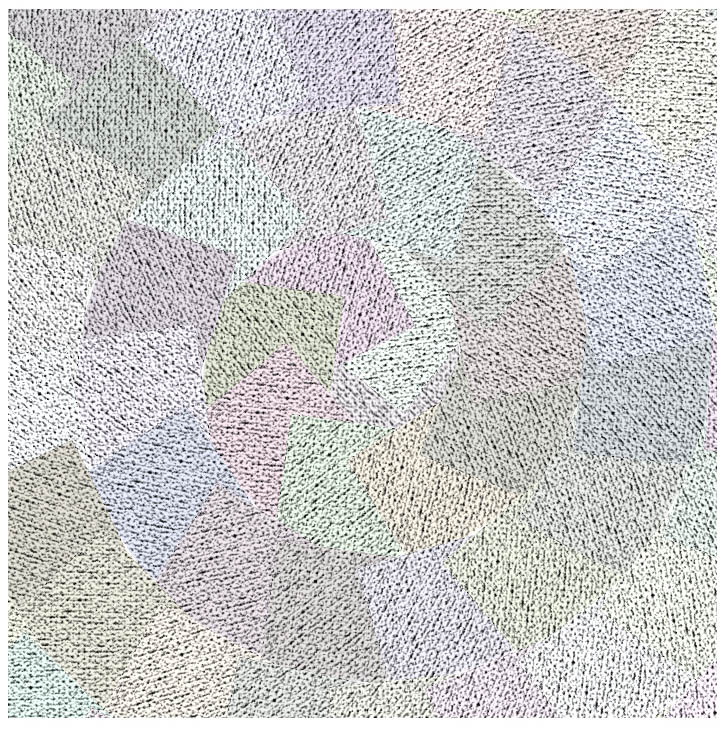
\includegraphics[width=0.5\textwidth]{figure_1.jpg}
		\caption{Add your figure caption here. \label{fig:example_fig}}		
	\end{center}
\end{figure}

You can reference a figure using the \textbf{\textbackslash{}ref\{\}}command. \textbf{Example:} see figure \ref{fig:example_fig}. To ensure accurate numbering of figures, place the \textbf{\textbackslash{}label\{\}} command inside the \textbackslash{}\{\}caption command of your figure. Below is an example of a second figure, using an EPS file as the graphic.

\begin{figure}[H]
	\begin{center}	
		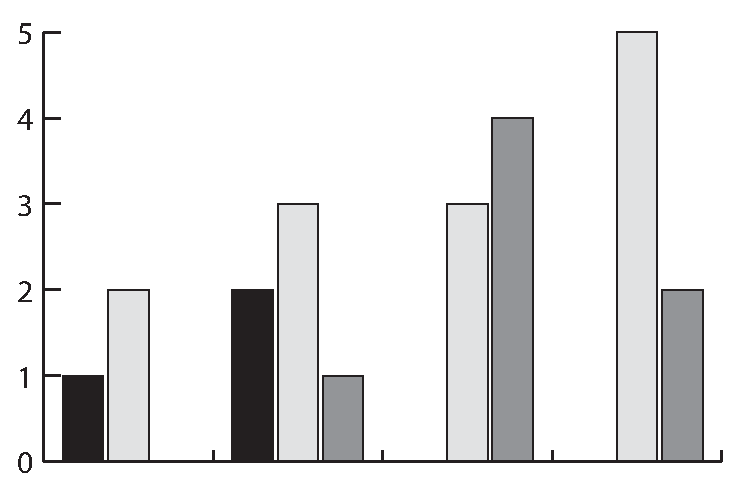
\includegraphics[width=0.5\textwidth]{figure_2.eps}
		\caption{A figure using an EPS graphic. \label{fig:example_fig2}}		
	\end{center}
\end{figure}

%%%%%%%%%%%%%%%%%%%%%%%%%%%%%%%%%%%
%%                               %%
%% Portraits                     %%
%%                               %%
%%%%%%%%%%%%%%%%%%%%%%%%%%%%%%%%%%%

\subsection{Portraits}

If your paper contains portraits of contributors, roundtable panelists, or interviewees where the portrait should be presented next to a brief bio or statement, please use the \textbf{ieeecsPortrait} enviroment. The portraits should align to the left with the bio wrapping around it on the right.

%{the name of your graphic}{the width of the graphic}{the text to wrap around the graphic}
\ieeecsPortrait{portrait.png}{0.25\textwidth}{The bio of the contributor should go here. This could also be a statement.}

%\vspace is used here since we have a very short bio and we want to make sure the next section starts after the portrait.
\vspace{7em}


\subsection{Tables}

Use the tabluar environment to build your table within \LaTeX. Tables require a title, added using the \textbf{\textbackslash{}caption\{\}} command. Tables are to be used to represent text in a tabular environment. Tables that are created as a graphic or contain graphics should instead use the figure environment.


%%%%%%%%%%%%%%%%%%%%%%%%%%%%%%%%%%%
%%                               %%
%% Table examples                %%
%%                               %%
%%%%%%%%%%%%%%%%%%%%%%%%%%%%%%%%%%%

\begin{table}[H]
	\begin{center}
		\caption{The table title goes here.\label{tab:example_tab}}
		\begin{tabular}{ |c|c|c|c| } 
			\hline
			col1 & col2 & col3 \\
			\hline
			\multirow{3}{4em}{Multiple row} & cell2 & cell3 \\ 
			& cell5 & cell6 \\ 
			& cell8 & cell9 \\ 
			\hline
		\end{tabular}
	\end{center}
\end{table}

\ieeecsTableFootnote{*If the table has a footnote add it after the table with the \textbf{ieeecsTableFootnote} command.}

\pagebreak
%\newnew page or \clearpage may be used to start a new page


\section{Distinct Article Elements}

\subsection{Algorithms}

Algorithms can be added by using lstlisting environment. Algorithms will have a thin frame around them and will be set in a monospace font. Algorithms require a caption and a label. Math can be added to algorithms using \LaTeX\ between the characters (\%* and \%*).


%LaTeX can be added in between the characters (%* and %*)
\begin{lstlisting}[caption={Add a caption for your algorithm here.}, label=Algorithm1]
1. Example of using lstlisting to write algorithms
2. (%*$\int\frac{d\theta} {1+\theta^2}=\tan^{-1} \theta+C$.%*)
...
10. End
\end{lstlisting}

\subsection{Program Code}

Program code should be added using the programCode environment. You can pass the language type as an optional parameter to properly style the code. Program code will not have a frame around it and will not have a caption.

Sample block of code formatted as PHP:

\begin{programCode}
[language=PhP]
$articleBaseName = basename($articleTeXFile, ".tex");
$articleXMLFile = basename($articleTeXFile, ".tex");
\end{programCode}


\subsection{Boxed Text}

%\ieeecsBoxedText{The ieeecsBoxed text environment can be used to set apart text ...}

\begin{ieeecsBoxedText}{The \textbf{ieeecsBoxedText} environment can be used to set apart text. Please pass the content of the boxed text as a parameter to this environment.}
\end{ieeecsBoxedText}


\subsection{Logos}

Popular logos related to \LaTeX~ are supported: \AllTeX\ \BibLaTeX\ \XeLaTeX\ \hologo{METAPOST}, and \hologo{METAFONT}.

%The command \ieeecsNonDisplayingText notes is provided as an option to include notes in your paper that will not be displayed. Pass text to both commands. This command will not display anything in the output.
\ieeecsNonDisplayingText{label}{Text} 

\section{References, Acknowledgements, and Author Bios}

A .bib file is required for your references. We will be using \BibTeX\ to compile the references of your paper. Please use \textbf{\textbackslash{}citep{}} to add citations to your paper. Examples \citep{Lamport1994a} and \citep{Goossens1997}. Please do not include footnotes or endnotes in your paper. \citep{Lamport1994a, Goossens1997}


%%%%%%%%%%%%%%%%%%%%%%%%%%%%%%%%%%%%%%%%%%%%%%%%%%%%%%%%%%%%%
%%                  Acknowledgments                        %%
%%                                                         %%
%%                                                         %%
%%%%%%%%%%%%%%%%%%%%%%%%%%%%%%%%%%%%%%%%%%%%%%%%%%%%%%%%%%%%%

\ieeecsAcknowledgmentsHeader{ACKNOWLEDGEMENTS}

\begin{ieeecsAcknowledgment}
Enter an acknowledgment here, within the \textbf{ieeeCSAcknowledgment} environment.
\end{ieeecsAcknowledgment}	

\newpage

%%%%%%%%%%%%%%%%%%%%%%%%%%%%%%%%%%%%%%%%%%%%%%%%%%%%%%%%%%%%%
%%                  The Bibliography                       %%
%%                                                         %%
%%                                                         %%
%%%%%%%%%%%%%%%%%%%%%%%%%%%%%%%%%%%%%%%%%%%%%%%%%%%%%%%%%%%%%

\ieeecsReferences{REFERENCES}

%Usage of the ieeeCSBib reference style file is required
\bibliographystyle{ieeeCSBib}

%change refs.bib to the name of your .bib file
\bibliography{refs}

%%%%%%%%%%%%%%%%%%%%%%%%%%%%%%%%%%%%%%%%%%%%%%%%%%%%%%%%%%%%%
%%                  Author Bios                            %%
%%                                                         %%
%%                                                         %%
%%%%%%%%%%%%%%%%%%%%%%%%%%%%%%%%%%%%%%%%%%%%%%%%%%%%%%%%%%%%%


\ieeecsAboutAuthor{ABOUT THE AUTHORS}


\begin{ieeecsAuthorBio}
\textbf{Author First and Last Name} is a [title or position] at [institution]. His/her research interests include [list here]. [Author last name] received a [highest degree] in [field of study] from [school]. Contact him/her at [preferred email address].
\end{ieeecsAuthorBio}

\begin{ieeecsAuthorBio}
	\textbf{Author First and Last Name} is a [title or position] at [institution]. His/her research interests include [list here]. [Author last name] received a [highest degree] in [field of study] from [school]. Contact him/her at [preferred email address].
\end{ieeecsAuthorBio}


\end{document}